\documentclass{article}
\usepackage{graphicx} % Required for inserting images
\usepackage{amsmath}
\usepackage{booktabs}
\usepackage{amssymb}
\usepackage{hyperref}
\usepackage{float} % Table placement

\title{Combinatorial Decision Making And Optimization}
\author{
  Cirone Cono, \texttt{cono.cirone@studio.unibo.it}
  \and
  Dardini Jacopo, \texttt{jacopo.dardini@studio.unibo.it}
  \and
  Formichella Gio, \texttt{gio.formichella@studio.unibo.it}
  \and
  Petrozziello Giulio, \texttt{giulio.petrozziello@studio.unibo.it} 
}
\date{}

\begin{document}

\maketitle


\section{Introduction}
% Add book reference
% Add complexity reduction analysis
In this project we tackle the sport scheduling problem with CP, SAT, SMT and MIP, and apply with all 4 technologies the common approach inspired by \cite{10.1007/10704567_6}. All implementations take as input the number of teams in the tournament and start by precomputing the weekly matchups for the round-robin tournament. The precomputation cost is minimal, for all tested team sizes the precomputation required less than a second. The matchup matrix not only speeds up the search by reducing the problem to ordering matchups, but also guarantees that the constraints of each team playing each other and playing once a week are satisfied. With all four techniques, we aim to find a solution satisfying the constraints and minimizing the objective variable D, the maximum difference between games played at home and away for a team; $D\in [1, n-1]$, where n is the number of teams.

\subsection{Notation}
\begin{itemize}
  \item $N$: number of teams
  \item $T=\{t\ |\ t \in [1, N]\}$: team identifiers
  \item $P=\{p\ |\ p \in [0, ..., \frac{N}{2} - 1]\}$: period identifiers
  \item $M=\{m\ |\ m \in [0, ..., \frac{N}{2} - 1]\}$: weekly matchup identifiers
  \item $W=\{w\ |\ w \in [0, ..., N-2]\}$: week identifiers
  \item $S=\{s\ |\ s \in [0,1]\}$: slot identifiers, where $s=0$ corresponds to playing at home and $s=1$ to playing away
  \item $rb_{m, w, s}=t$: team $t$ plays in week $w$ in match $m$ in slot $s$.
  % \item $m=rb_{p, w}$ is the match $(t_1, t_2)$ in period $p$ of week $w$, where $t_1$ plays at home and $t_2$ plays away
  
\end{itemize}

\section{CP Model}
\subsection{Decision Variables}
This model utilizes two primary decision variables to construct the tournament schedule and assign home/away teams for each match.

\subsubsection{\text{matches}}
The variable $\text{matches}_{p, w} \in [0, \dots, \frac{N}{2} - 1]$ for $p \in P, w \in W$, determines which match from the predefined round-robin structure ($\text{rb}$) is scheduled in week $w$ and period $p$.

\subsubsection{\text{home\_away}}
The binary variable $\text{home\_away}_{p, w} \in \{0, 1\}$ for $p \in P, w \in W$, assigns the home team for the match scheduled at period $p$ in week $w$. Specifically, $\text{home\_away}_{p, w} = 0$ means the first team listed in the match plays at home, while $\text{home\_away}_{p, w} = 1$ means the second team plays at home.

\subsection{Auxiliary Variables}
\subsubsection{\text{home\_games}}
The auxiliary variable $\text{home\_games}_{t} \in [1, \dots, N-1]$ for $t \in T$, represents the total number of home games assigned to team $t$ throughout the tournament. Its value is derived from the assignments of the decision variables $\text{matches}$ and $\text{home\_away}$.


\subsection{Objective Function}

The model's objective is to quantify and minimize disparities in home game assignments through the $\text{max\_imbalance}$ variable.

\subsubsection{Objective Variable: \text{max\_imbalance}}\label{objective}
The integer variable $\text{max\_imbalance} \in [1, \dots, N-1]$ quantifies the maximum absolute disparity in home game assignments across all teams. The lower bound of 1 acknowledges that perfect balance ($\text{max\_imbalance}=0$) is not achievable for an odd number of total games ($N-1$ games). The upper bound of $N-1$ represents the theoretical maximum possible deviation, occurring if a team plays all its games either at home or away.

The value of $\text{max\_imbalance}$ is determined by the following fairness constraint:
\[ \forall t \in T : \left| 2 \times \text{home\_games}_{t} - (N-1) \right| \leq \text{max\_imbalance} \]
This formulation precisely defines the absolute "imbalance" for each team $t$. This imbalance is derived from the difference between a team's home games and away games. Since $\text{home\_games}_{t} + \text{away\_games}_{t} = N-1$ (total games), substituting the expression for $\text{away\_games}_{t}$ yields the imbalance for team $t$ as $2 \times \text{home\_games}_{t} - (N-1)$. By enforcing that the absolute value of this imbalance for every team must be less than or equal to $\text{max\_imbalance}$, this variable effectively captures the largest such deviation among all teams, serving as the direct measure of the overall schedule's fairness.


\subsubsection{Objective}
The objective is to \textbf{minimize $\text{max\_imbalance}$}:
\[ \text{minimize } \text{max\_imbalance} \]
This aims to achieve the fairest possible distribution of home and away games. An optimal solution would ideally yield $\text{max\_imbalance}=1$, meaning each team's home/away game count differs by at most one, which is the best possible outcome for an odd number of total games played.


\subsection{Constraints}
\subsubsection{Core Constraints}
These constraints are strictly necessary for defining a feasible round-robin schedule:
\begin{enumerate}
    \item \textbf{Each period must be used exactly once per week:} Ensures that for every week, all matches generated by the round-robin structure's periods are indeed scheduled. Without this, some pairings might be missed, or periods might be duplicated, leading to an incomplete or invalid schedule.
    \[ \forall w \in W : \texttt{all\_different}([\texttt{matches}[p, w] \mid p \in P]) \]

    \item \textbf{Each team plays at most twice per period:} 
\[ \forall p \in P, \forall t \in T : \left| \{ (w, s) \mid w \in W, s \in S, \text{rb}_{\text{matches}_{p, w}, w, s} = t \} \right| \leq 2 \]

 \item \textbf{Calculation of Home Games:} This constraint defines the value of $\text{home\_games}_{t}$.
\[ \forall t \in T : \text{home\_games}_{t} = \sum_{p \in P, w \in W, s \in S} \mathbb{I}\left( \text{rb}_{\text{matches}_{p, w}, w, s} = t \land \text{home\_away}_{p, w} = s \right) \]
The indicator function $\mathbb{I}(\cdot)$ ensures that 1 is added to the sum if team $t$ is located in slot $s$ and that slot $s$ is designated as the home slot by $\text{home\_away}_{p,w}$.



    \item \textbf{Fairness - balance home and away games:} This constraint directly links the calculated $\text{home\_games}$ for each team to the objective variable $\text{max\_imbalance}$. For a detailed explanation of this relationship and the definition of $\text{max\_imbalance}$, please refer to Section \ref{objective} (Objective Variable and Objective Function).
    
    
\end{enumerate}

\subsubsection{Implied Constraints}

\begin{enumerate}
    \item \textbf{Each team appears exactly once per week:}
    \[ \forall w \in W, \forall t \in T : \left| \{ (p, s) \mid p \in P, s \in S, \text{rb}_{\text{matches}_{p, w}, w, s} = t \} \right| = 1 \]
\end{enumerate}

\subsubsection{Symmetry Breaking Constraints}

\begin{enumerate}
    \item \textbf{Break period assignment symmetry using lexicographic ordering:} The order in which matches corresponding to $P$ are assigned within $\text{matches}$ for each week is symmetrical. This constraint breaks such symmetries by enforcing a lexicographical ordering, reducing the number of equivalent search paths.
    \[ (\text{matches}_{p, w})_{p \in P, w \in W} \succeq_{\text{lex}} (\text{matches}_{p, w})_{\text{reversed}(p) \in P, w \in W} \]
    This states that the sequence of $\text{matches}$ variables, when read in normal $(p,w)$ order, must be lexicographically greater than or equal to when read in $(p,w)$ order with $p$ reversed. This helps to fix one permutation of period assignments.

    \item \textbf{Fix first match home assignment to break home/away symmetry:} This constraint eliminates global home/away assignment symmetry by fixing the home/away status of the first match.
    \[ \text{home\_away}_{0, 0} = 0 \]

\item \textbf{Balance the home/away assignments within each week:} While not a strict symmetry breaking constraint, this constraint helps reduce the search space by ensuring that within each week $w$, the number of matches where the second team plays at home ($\text{home\_away}_{p, w}=1$) is roughly half of the total matches ($|P|$), with a maximum deviation of 1:
\[ \forall w \in W : \left| \sum_{p \in P} \text{home\_away}_{p, w} - \left\lfloor \frac{|P|}{2} \right\rfloor \right| \leq 1 \]
This guides the solver towards balanced assignments and prunes highly imbalanced weekly configurations.

\end{enumerate}

\subsection{Validation}

The model was implemented in MiniZinc and validated through a series of experiments designed to assess solver performance under various model configurations and search strategies.

\subsubsection{Experimental Design}

To comprehensively evaluate the performance of different solving strategies for the Sports Tournament Scheduling problem, a systematic experimental study was conducted.

\textbf{Hardware and Software:}
Experiments were executed on a MacBook Air M1 equipped with an 8-core CPU. The following solvers were employed: \textit{Gecode}, \textit{Chuffed} and \textit{OR-Tools CP-SAT}. 
A uniform time limit of $300$ seconds was imposed for each individual problem instance.

\textbf{Model Configurations:}
Four configurations were tested: \texttt{baseline (core)}, \texttt{baseline+implied}, \texttt{baseline+symmetry breaking}, \texttt{full model}.

\textbf{Search Strategies:}
Three distinct search strategies were employed to analyze solver behavior, with a particular focus on how they influenced Gecode, often considered to have weaker default heuristics compared to modern SAT-based solvers.

\textbf{Search Strategies:}
Three distinct search strategies were employed to analyze solver behavior, focusing on their influence on Gecode, given its often weaker default heuristics compared to modern SAT-based solvers.

\begin{enumerate}
    \item \textbf{Default Search Strategy (Solver's Default):} Each solver relied entirely on its built-in decision heuristics and restart policies, serving as a baseline for their inherent capabilities.

    \item \textbf{Sequential Custom Search Strategy:} A manually defined sequential search (\texttt{seq\_search}) was applied, prioritizing \texttt{matches} variables with \texttt{dom\_w\_deg} and \texttt{home\_away} variables with \texttt{first\_fail}, utilizing a \texttt{restart\_luby(100)} policy.

    \item \textbf{Relax-and-Reconstruct (LNS) Strategy:} This higher-level strategy incorporated \texttt{relax\_and\_reconstruct} on the \texttt{matches} variables (preserving 60\% of solution values), leveraging Large Neighborhood Search (LNS) techniques. It was layered on top of the "Sequential Custom Search Strategy."
\end{enumerate}

\textbf{Solver-Specific Strategy Application:}
To ensure a fair and controlled comparison under single-threaded conditions (aligning with project constraints), OR-Tools CP-SAT was run without multi-threading. For both Chuffed and OR-Tools CP-SAT, the \texttt{free\_search} parameter was explicitly omitted when applying the custom Sequential Custom Search and Relax-and-Reconstruct strategies. This allowed direct evaluation of the user-defined MiniZinc search annotations, rather than the solvers' highly optimized default heuristics.


\subsubsection{Experimental Results}
\begin{table}[htbp]
\centering
\small
\resizebox{\textwidth}{!}{%
\begin{tabular}{c|cccc|cccc|cccc}
\toprule
\textbf{n} & \multicolumn{4}{c|}{\textbf{GECODE}} & \multicolumn{4}{c|}{\textbf{CHUFFED}} & \multicolumn{4}{c}{\textbf{CP-SAT}} \\
\cmidrule(lr){2-5}\cmidrule(lr){6-9}\cmidrule(lr){10-13}
  & bs & complete & noIMPL & noSB & bs & complete & noIMPL & noSB & bs & complete & noIMPL & noSB \\
\midrule
6 & 0 & 0 & 0 & 0 & 0 & 0 & 0 & 0 & 0 & 0 & 0 & 0 \\
8 & 6 & 6 & 6 & 6 & 0 & 0 & 0 & 0 & 0 & 0 & 0 & 0 \\
10 & N/A & N/A & N/A & N/A & 0 & 0 & 0 & 0 & 1 & 1 & 1 & 1 \\
12 & N/A & N/A & N/A & N/A & 60 & 6 & 5 & 6 & 4 & 3 & 3 & 3 \\
14 & N/A & N/A & N/A & N/A & 175 & 175 & 180 & 194 & 5 & 5 & 5 & 5 \\
16 & N/A & N/A & N/A & N/A & N/A & N/A & N/A & N/A & 15 & 15 & 15 & 15 \\
18 & N/A & N/A & N/A & N/A & N/A & N/A & N/A & N/A & 273 & 265 & 265 & 265 \\
20 & N/A & N/A & N/A & N/A & N/A & N/A & N/A & N/A & 85 & 84 & 84 & 84 \\
22 & N/A & N/A & N/A & N/A & N/A & N/A & N/A & N/A & 239 & 226 & 247 & 218 \\
\bottomrule
\end{tabular}%
}
\caption{CPU time in seconds for finding the \textit{optimal solution} using \textit{Default Search Strategy (Solver's Default)}}
\end{table}

\begin{table}[htbp]
\centering
\small
\resizebox{\textwidth}{!}{%
\begin{tabular}{c|cccc|cccc|cccc}
\toprule
\textbf{n} & \multicolumn{4}{c|}{\textbf{GECODE}} & \multicolumn{4}{c|}{\textbf{CHUFFED}} & \multicolumn{4}{c}{\textbf{CP-SAT}} \\
\cmidrule(lr){2-5}\cmidrule(lr){6-9}\cmidrule(lr){10-13}
  & bs & complete & noIMPL & noSB & bs & complete & noIMPL & noSB & bs & complete & noIMPL & noSB \\
\midrule
6 & 0 & 0 & 0 & 0 & 0 & 0 & 0 & 0 & 0 & 0 & 0 & 0 \\
8 & 0 & 0 & 0 & 0 & 0 & 0 & 0 & 0 & 0 & 0 & 0 & 0 \\
10 & 0 & 0 & 0 & 0 & 0 & 0 & 0 & 0 & 1 & 1 & 1 & 1 \\
12 & 0 & 0 & 0 & 0 & 0 & 0 & 0 & 0 & 55 & 56 & 58 & 48 \\
14 & 4 & 7 & 4 & 7 & N/A & 53 & 34 & N/A & N/A & N/A & N/A & N/A \\
16 & N/A & N/A & 191 & 164 & N/A & N/A & N/A & N/A & N/A & N/A & N/A & N/A \\
\bottomrule
\end{tabular}%
}
\caption{CPU time in seconds for finding the \textit{optimal solution} using \textit{Sequential Custom Search Strategy}}
\end{table}

\begin{table}[htbp]
\centering
\small
\resizebox{\textwidth}{!}{%
\begin{tabular}{c|cccc|cccc|cccc}
\toprule
\textbf{n} & \multicolumn{4}{c|}{\textbf{GECODE}} & \multicolumn{4}{c|}{\textbf{CHUFFED}} & \multicolumn{4}{c}{\textbf{CP-SAT}} \\
\cmidrule(lr){2-5}\cmidrule(lr){6-9}\cmidrule(lr){10-13}
  & bs & complete & noIMPL & noSB & bs & complete & noIMPL & noSB & bs & complete & noIMPL & noSB \\
\midrule
6 & 0 & 0 & 0 & 0 & 0 & 0 & 0 & 0 & 0 & 0 & 0 & 0 \\
8 & 0 & 0 & 0 & 0 & 0 & 0 & 0 & 0 & 0 & 0 & 0 & 0 \\
10 & 0 & 0 & 0 & 0 & 0 & 0 & 0 & 0 & 1 & 1 & 1 & 1 \\
12 & 0 & 0 & 0 & 0 & 9 & 1 & 3 & 2 & 56 & 62 & 59 & 52 \\
14 & 1 & 5 & 1 & 0 & N/A & 89 & 187 & 258 & N/A & N/A & N/A & N/A \\
16 & 184 & 19 & 1 & 8 & N/A & N/A & N/A & N/A & N/A & N/A & N/A & N/A \\
18 & N/A & 3 & N/A & N/A & N/A & N/A & N/A & N/A & N/A & N/A & N/A & N/A \\
\bottomrule
\end{tabular}%
}
\caption{CPU time in seconds for finding the \textit{optimal solution} using \textit{Relax-and-Reconstruct (LNS) Strategy}}
\end{table}

% TODO:
% - explain constraint encoding (Heule, sequential)
% - correct results in tables
% - add auxiliary variables
% - add versioning
% - add hardware specs to introduction and remove other occurrences
\section{SAT Model}
\subsection{Decision variables}
Let $sts$ be a schedule analogous to $rb$ satisfying to the STS problem:
% The satisfiability task is formalized by the following categories of propositions:

\subsubsection{Satisfiability}
% \paragraph{\text{matches\_schedule}}
\begin{itemize}
    \item \textbf{matches\_schedule}\\
        For each period $p \in P$ and week $w \in W$:
        $$
        matches\_schedule_{p, w, m} = true
        $$
        if, and only if, the match $rb_{m, w}$ takes place in period $p$ of week $w$
    \item \textbf{matches\_to\_periods}\\
        For each period $p \in P$, $t_1 \in T$ and $t_2 \in T/\{t_1\}$:
        $$
        matches\_to\_periods_{t_1, t_2, p} = true
        $$
        if, and only if, $t_1$ plays against $t_2$ in period $p$
\end{itemize}
\subsubsection{Optimization}
\begin{itemize}
    \item \textbf{flip\_slot}\\
        For each period $p \in P$ and week $w \in W$:
        $$
        flip\_slot_{p, w} = true
        $$
        if, and only if, team $sts_{p, w, 1} = t_1$ plays away
    \item \textbf{matches\_to\_slots}\\
        For each period $p \in P$, $t_1 \in T$ and $t_2 \in T/\{t_1\}$:
        $$
        matches\_to\_slots_{t_1, t_2} = true
        $$
        if, and only if, $t_1$ plays away and $t_2$ plays at home
\end{itemize}

\subsection{Objective function}
Similarly to the other approaches, the objective is to minimize the absolute difference between the number of games played at home and away for each team.
Let $A_t$ be the number of times the team $t \in T$ plays away, the objective function translates into the following:
$$
k^* = \underset{k \in \mathbb{N}}{\text{argmax}} \left( \forall t \in T, A_t \geq k \right)
$$
The chosen model allows to solve the optimization task using the $sts$ schedule computed in the satisfiability process. The optimization consists of a binary search of $k^*$ in the interval $[1, \lfloor\frac{N-1}{2}\rfloor]$. Since SAT doesn't directly support optimization, a new set of optimizing constraints is introduced for every instance of $k$ .

The result is encoded in $flip\_slot_{p, w}$, which cannot express the constraints alone, due to structural limitations of the encoding.
Instead \\$matches\_to\_slots_{t_1, t_2}$ is used: given a week $w$ and a period $p$, the team $sts_{p, w, 1} = t_1$ plays away if, and only if, the team $t_2 = sts_{p, w, 2}$ plays at home. Therefore, by definition:
$$
    \forall p \in P, w \in W.(flip\_slot_{p, w} \leftrightarrow matches\_to\_slots_{sts_{p, w, 1}, sts_{p, w, 2}})
$$
Finally the optimization process is implemented by ensuring that for an instance $k \in [1, \lfloor\frac{N-1}{2}\rfloor]$:
$$
    \forall p \in P, t_1 \in T.(AtLeastK(matches\_to\_slots_{t_1, t_2} | t_2 \in T/\{t_1\}))
$$

\subsection{Constraints}
\subsubsection{Each match is assigned to a unique period each week}
In a Round-Robin tournament $rb$, each team plays exactly once a week. 
Therefore the only problem is to ensure that for each week $w$, every match $rb_{m, w} = (t_i, t_j)$ is assigned to exactly one period $p$.

We enforce that every match is scheduled once:
$$
    \forall p \in P, w \in W.(ExactlyOne(matches\_schedule_{p, w, m} | m \in P))
$$
Finally no two matches are scheduled in the same period. 

We ensure that each match is scheduled to a unique period $p$ in the week $w$.
$$
    \forall m \in P, w \in W. ExactlyOne(matches\_schedule_{p, w, m} | p \in P)
$$
\subsubsection{Every team plays at most twice in the same period}
The constraint cannot be expressed using directly $matches\_schedule_{p, w, m}$, due to structural limitations of the encoding. 
Instead, we introduce the literal $matches\_to\_periods_{t_1, t_2, p}$: given a week $w$, the match $rb_{m,w}$ is scheduled in period $p$ if, and only if, the match $(rb_{m, w, 1}, rb_{m, w, 2}) = (t_1, t_2)$ takes place in period $p$. Therefore, by definition: 
$$
    \forall p \in P, w \in W, m \in P.(matches\_schedule_{p, w, m} \leftrightarrow matches\_to\_periods_{rb_{m, w, 1}, rb_{m, w, 2}, p})
$$
Computationally this constraint soundly binds $matches\_schedule$ to \\$matches\_to\_periods$, which allow to express the main constraint:
$$
    \forall p \in P, t_1 \in T. AtMost2(matches\_to\_periods_{t_1, t_2, p} | t_2 \in T/\{t_1\})
$$
\subsection{Validation}
% See Section 2.4. The model \textbf{must} be implemented using at least Z3. Bonus points will be considered if a solver-independent language (e.g., Dimacs) is employed so as to play with different SAT solvers on the same model.
\subsubsection{Experimental design}
The model was written in Python by making use of the Z3 and the CVC5 library, which offers CaDiCaL and MiniSat as the underlying SAT solvers. The time elapsed to find an optimal solution, within the 300 second time limit, was measured and results presented in Fig.\ref{fig:SAT-result} . 
\subsubsection{Experimental results}
All solvers either find the optimal solution or no solution at all. Overall Z3 had the fastest and was able to solve the problems with higher $N$, reaching $N=20$. On the other hand CaDiCaL was the worst, failing at $N=12$, while MiniSat stopped at $N=14$

\begin{table}[H]
\centering
\small
{%
\begin{tabular}{|c|c|c|c|}
\toprule
\textbf{n} & \textbf{Z3} &\textbf{CaDiCaL} & \textbf{MiniSat} \\
\midrule
6  & 0   & 0   & 0   \\
8  & 0   & 0   & 0   \\
10 & 0   & 0   & 0   \\
12 & 0   & N/A & N/A \\
14 & 0   & N/A & N/A \\
16 & 1   & N/A & N/A \\
18 & 16  & N/A & N/A \\
20 & 221 & N/A & N/A \\
22 & N/A & N/A & N/A \\
\bottomrule
\end{tabular}
}
\caption{SAT optimization solver results}
\label{table:mip-results}
\end{table}

% \begin{figure}[H]
%     \centering
%     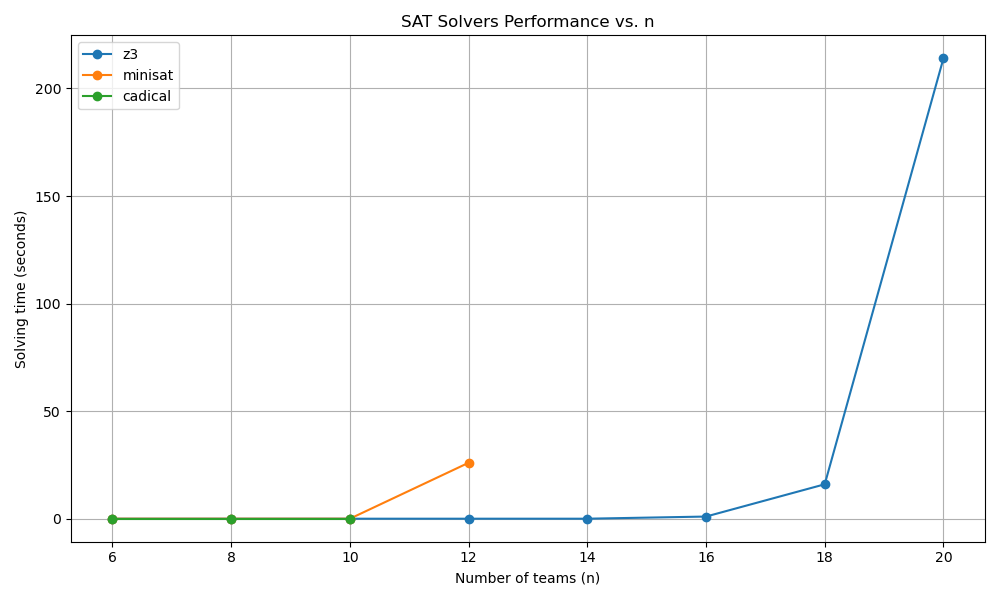
\includegraphics[width=0.8\linewidth]{img/SAT-result.png}
%     \caption{SAT optimization}
%     \label{fig:SAT-result}
% \end{figure}


\section{SMT Model}

\subsection{Decision Variables}

The SMT model is divided into two phases:

\begin{itemize}
    \item \textbf{Phase~1}: selects exactly one match pair $m$ for each period $p$ and week $w$.
    \item \textbf{Phase~2}: reuses the feasible schedule and flips home/away slots to optimize balance.
\end{itemize}

\textbf{Phase~1 variables}:
\begin{itemize}
    \item $\mathit{index}_{p,w,m} \in \{\text{true}, \text{false}\}$: true if match pair $m$ is selected for $(p,w)$.
    \item $\mathit{home}_{p,w} \in T$: home team in $(p,w)$.
    \item $\mathit{away}_{p,w} \in T$: away team in $(p,w)$.
\end{itemize}

\textbf{Phase~2 variables}:
\begin{itemize}
    \item $\mathit{flip}_{p,w} \in \{\text{true}, \text{false}\}$: indicates if match in $(p,w)$ is flipped.
    \item $\mathit{homeEff}_{p,w}$, $\mathit{awayEff}_{p,w}$: effective teams after flipping.
\end{itemize}

\subsection{Objective Function}

Minimize the maximum imbalance $k$:
\[
k^* = \min \Big\{ k ~|~ \forall t \in T: |H_t - A_t| \leq k \Big\},
\quad 
H_t = \sum_{p,w} [\, \mathit{homeEff}_{p,w} = t\,], \quad 
A_t = \sum_{p,w} [\, \mathit{awayEff}_{p,w} = t\,].
\]

Effective teams:
\[
\mathit{homeEff}_{p,w} = \text{ite}(\mathit{flip}_{p,w}, \mathit{away}_{p,w}, \mathit{home}_{p,w}), 
\quad
\mathit{awayEff}_{p,w} = \text{ite}(\mathit{flip}_{p,w}, \mathit{home}_{p,w}, \mathit{away}_{p,w}).
\]

\subsection{Constraints}

\subsubsection{Unique match assignment per slot}

Each period $(p,w)$ must select exactly one match pair:
\[
\forall p \in P,\, w \in W:\; 
\sum_{m \in M} \mathit{index}_{p,w,m} = 1.
\]

\subsubsection{Each match pair used exactly once per week}

Each pair $m$ must be assigned exactly once within each week:
\[
\forall m \in M,\, w \in W:\; 
\sum_{p \in P} \mathit{index}_{p,w,m} = 1.
\]

\subsubsection{Binding decision}

If $\mathit{index}_{p,w,m}$ is true, the slot must bind to $rb$:
\[
\forall p \in P,\, w \in W:\; 
\bigvee_{m \in M} \Big(
  \mathit{index}_{p,w,m} \wedge 
  \mathit{home}_{p,w} = rb_{m,w,0} \wedge 
  \mathit{away}_{p,w} = rb_{m,w,1}
\Big).
\]

\subsubsection{Team appears at most twice in same period}

A team cannot appear more than twice in the same period over the whole tournament:
\[
\forall t \in T,\, p \in P: 
\sum_{w \in W} 
\sum_{m \in M} \Big(
  [\, rb_{m,w,0} = t \vee rb_{m,w,1} = t\, ] \cdot [\, \mathit{index}_{p,w,m} \, ]
\Big) 
\leq 2.
\]

\subsubsection{Symmetry breaking}

Fix first match pair in first slot:
\[
\mathit{index}_{0,0,0} = \text{true}.
\]

\subsubsection{Imbalance constraint}

For Phase~2:
\[
|H_t - A_t| \leq k.
\]

\subsection{Validation}

\subsubsection{Experimental design}

Implemented in Python + SMT-LIB. Solvers: Z3 and CVC5, timeout 300s. Phase~1 finds feasible solution; Phase~2 binary-searches the minimal $k$.

\subsubsection{Results}

Z3 solves larger instances faster. CVC5 is feasible for small $N$ only.

\begin{figure}[h!]
  \centering
  \includegraphics[width=0.8\linewidth]{output.png}
  \caption{SMT solution example}
  \label{fig:smt-result}
\end{figure}

\begin{table}[htbp]
\centering
\small
\begin{tabular}{|c|c|c|}
\toprule
\textbf{n} & \textbf{Z3 (s)} & \textbf{CVC5 (s)} \\
\midrule
6  & 0.11 & 0.13 \\
8  & 0.17 & 1.85 \\
10 & 0.23 & N/A \\
12 & 0.29 & N/A \\
14 & 0.36 & N/A \\
16 & 0.74 & N/A \\
18 & 3.52 & N/A \\
20 & 14.32 & N/A \\
22 & 280.17 & N/A \\
24 & N/A & N/A \\
\bottomrule
\end{tabular}
\caption{SMT solving times}
\label{table:smt-result}
\end{table}


\section{MIP}
\subsection{Decision variables}
\subsubsection{match\_schedule}
For each $w \in W$ and $p \in P$, the binary
$$
match\_schedule_{w,p,m} = 1
$$
if, and only if, in week $w$ and period $p$ match $m \in M$ is played 

\subsubsection{flip\_slot}
For each week $w \in W$ and period $p \in P$  
$$  
flip\_slot_{w,p} = a \in \{0, 1\}  
$$  
determines which team from match $rb_{p, w} = (t_1, t_2)$ in week w and period p is assigned as the home team. Specifically, $a = 0$ means $t_1$ plays at home and $t_2$ away, while $a = 1$ means the assignment is reversed.

\subsubsection{team periods of play}
For each $t \in T$, $w \in W$ and $p \in P$, the binary
$$
TP_{t,w,p} = 1
$$
if, and only if, team t plays in week w and period p.

\subsubsection{home games counter}
For each team $t \in T$, the integer  
$$  
H_t = h \in [1, \dots, N-1]
$$  
determines the total number of home games assigned to team $t$ throughout the tournament.

\subsection{Objective Function}
The model's objective is to minimize the maximum absolute difference between the number of home and away games played by any team. This maximum difference is quantified by the integer variable $D \in [1, \dots, N-1]$, which was previously referred to as $\text{max\_imbalance}$. We first find, for each team, the number of games played at home (2), and then constrain D as being greater or equal than the difference of home and away games for each team. Given that we have a minimization problem, this is effectively equivalent to computing the max: 
$$\begin{cases}
    \min d \\
    d = \max_t |home_t - away_t|
\end{cases} = \begin{cases}
    \min d \\
    d \geq |home_t - away_t| \ \forall t \in T
\end{cases}$$The absolute value of the difference is not computed explicitly but is decomposed into 2 inequalities (3)(4). Finally, we look for the minimum of D (1).

\begin{align}
    \min \ &D \\
    H_t =& \sum_{w \in W, m \in M} \mathbbm{1}[flip\_slot_{w,p} = 0 \land rb_{m,w,0} = t] \notag \\
    +& \sum_{w \in W, m \in M} \mathbbm{1}[flip\_slot_{w,p} = 1 \land rb_{m, w,1} = t] \hspace{20px}  && \forall t \in T\\
    D &\geq 2H_t - (N-1) && \forall t \in T\\
    D & \geq -(2 H_t - (N-1)) && \forall t \in T
\end{align}

\subsection{Constraints}
\subsubsection{Each match is assigned to a unique period each week}
Due to how the decision variables are defined, it was necessary to impose that each period in each week is assigned a single match (5) and each match is assigned to a single period (6).

\begin{align}
    \sum_{m \in M} match\_schedule_{w,p,m} &= 1 \hspace{20px} \forall p \in P \hspace{10px} \forall w \in W\\
    \sum_{p \in P} match\_schedule_{w,p,m} &= 1 \hspace{20px} \forall m \in M \hspace{10px}\forall w \in W
\end{align}

\subsubsection{Each team plays at most twice in the same period}
The constraint on teams playing at most twice in the same period is imposed by first linking the variables of $match\_schedule$ to those in TP based on the values in $rb$ (7) and then limiting the sum of periods of play to being smaller or equal than 2 (8). 

\begin{align}
    TP_{t,w,p} &= match\_schedule_{w,p,m} \hspace{20px} \text{where}\ t \in rb_{m, w} \hspace{20px} \forall t \forall p  \forall w\\
    \sum_{w \in W} &TP_{t,w,p} \leq 2 \hspace{40px} \forall t \in T \hspace{10px} \forall p \in P
\end{align}

\subsection{Validation}
\subsubsection*{Experimental design}
The model is written in Python by making use of the PuLP library. The solvers tested on the model were: CBC 2.10.3, HiGHS 1.10.0, CPLEX 22.1.1 and SCIP 5.5.0, all used with their default parameters. The time elapsed to find an optimal solution, within the 300 second time limit, was measured for each solver up to N=24. All tests were run on a single core of an Intel i7-10750H CPU.

\subsubsection*{Experimental results}
As shown in Table \ref{table:mip-results}, CBC had the worst performance, it isn't able to find the optimal solution for n greater than 14. CPLEX, instead, is the fastest up to N=14 but after N=16 it stops finding a solution. HiGHS was able to find an optimal schedule up to N=18 and SCIP, the best performer of the four, was able to reach N=20.

\begin{table}[htbp]
\centering
\small
{%
\begin{tabular}{|c|c|c|c|c|}
\toprule
\textbf{N} & \textbf{CBC} &\textbf{HiGHS} & \textbf{CPLEX} & \textbf{SCIP} \\
\midrule
6 & 0 & 0 & 0 & 0 \\
8 & 0 & 0 & 0 & 0 \\
10 & 1 & 0 & 0 & 0 \\
12 & 2 & 1 & 0 & 5 \\
14 & 45 & 12 & 5 & 17\\
16 & N/A & 62 & 20 & 15\\
18 & N/A & 218 & N/A & 192\\
20 & N/A & N/A & N/A & 101\\
22 & N/A & N/A & N/A & N/A\\
\bottomrule
\end{tabular}
}
\caption{MIP optimization solver results}
\label{table:mip-results}
\end{table}

It was also verified that the solvers either find an optimal solution or no solution at all within the time limit.

\bibliographystyle{unsrt}
\bibliography{ref.bib}

\end{document}
